%Define the timeline: is a step where the overall schedule for the project is estimated. There are two starting points for this: 1) Flexible ending (i.e., flexible investments and flexible functionality) and 2) Fixed ending. The latter one is described in the variant section of this pattern. In Agile software development the situation may often be that the finishing time of the project is dependent on the completion of the product (due to the constantly changing/involving requirements). Thus, a clear timeline can not be set but rather estimations.

Inicialmente se define una linea temporal cuya fecha de inicio es la concepción de la idea y la primera entrevista de elicitación de requisitos. La idea del proyecto fue concebida por el autor el día \textit{5 de noviembre del 2013}. Posteriormente la entrevista se realizó el \textit{jueves 21 de noviembre de 2013}. Una vez realizada la entrevista se contactó con la tutora del proyecto, se le expuso la idea y se le hizo entrega de una transcripción de la entrevista; dicho primer encuentro se llevó a cabo \textit{el martes 10 de diciembre de 2013}. \\

Se toma como fecha de inicio la fecha en la cual se comenzó a desarrollar el documento, la formación, definición de objetivos,planificación y desarrollo del proyecto. Por lo tanto se considera como \textbf{fecha de incicio} el día \textit{5 de enero de 2014}. \\
 
%Define the rhythm: is a step where the lengths and number (estimated) of the iterations (i.e., product releases) is set. This also included the identification of other main checkpoints (i.e., milestones) related to, for example, quality assurance issues.
El ritmo de entrega una vez comience el desarrollo se tratará de que sea cada dos semanas. Éstas iteraciones siempre que sea posible serán enviadas para su evaluación al \textit{Auditor Externo}. \\

%Define/estimate the investments: is a step where the interest groups commonly agree on the costs of the project; the effort and financial investments for the product development. However, considering the flexible ending of the project, these investments may be highly dependent on the changes on, for example, requirements. Some decisions, however, need to be established concerning the estimations as well as their possible revision later on.
Aunque en el momento de inicio del proyecto se desconoce la fecha exacta de exposición se ha establecido que se llevará a cabo entre los meses de junio y julio. Por lo que, a efectos de planificación, se impondrá como \textbf{fecha de finalización} del proyecto el día \textit{1 de junio de 2014}. Esta fecha de final tiene cierta flexibilidad, dado en cuanto se conozca la fecha exacta de exposición del pfg se podrá modificar la planificación en función de ello. \\

En la etapa de \textbf{Inicializar} se llevará a cabo un largo periodo de formación en el que se investigarán las tecnologías a emplear, así como el manejo del os lenguajes y herramientas, para dicha formación a priori se asignarán unos 32 días. Seguidamente se procederá a planificar la arquitectura y seguidamente a realizar el análisis de la requisitos. Con todo ello se comenzará el proceso de Produccionizar en el que se estiman 4 iteraciones. En la primera iteración se desarrollara la app móvil con todas las funcionalidad a excepción de la funcionalidad que comunica con el servidor. Seguidamente se desarrollará el servidor con su correspondiente base de datos, y un software para consultas y resolución de peticiones anómalas. Finalmente se elaborarán un servicio que permita ejercer de intermediario entre las peticiones de los terminales móvil y el servidor de forma segura. Finalmente se implementará la funcionalidad en la app para dispositivo móvil. Se estima que dada la naturaleza de la aplicación se estima un mayor tiempo al desarrollo de la app móvil que al servidor y al servicio estimando un plazo de 21 días para el desarrollo de la app móvil inicial y unos 7 días para incluir la funcionalidad que comunicará con el proveedor de servicio para las peticiones al servidor.  \\

Posteriormente se realizarán 2 semanas de pruebas de integración en la etapa de \textbf{Estabilizar} y finalmente 19 días para \textbf{Test y reparación del Sistema}. Durante todo el proceso de elaboración del proyecto en todas las etapas va implícita la realización de la documentación reflejando las distintas tareas llevadas a cabo en cada una de ellas. Una vez finalizado el proyecto y realizada la documentación correspondiente, el tiempo restante hasta la exposición será empleado en la preparación y ensayó de una presentación y una prueba de cara al tribunal de evaluación. \\

% Diagrama de Gantt
Se adjunta a continuación el diagrama de Gantt generado para plasmar la planificación del proyecto. 

\begin{figure}[H]
  \centering
  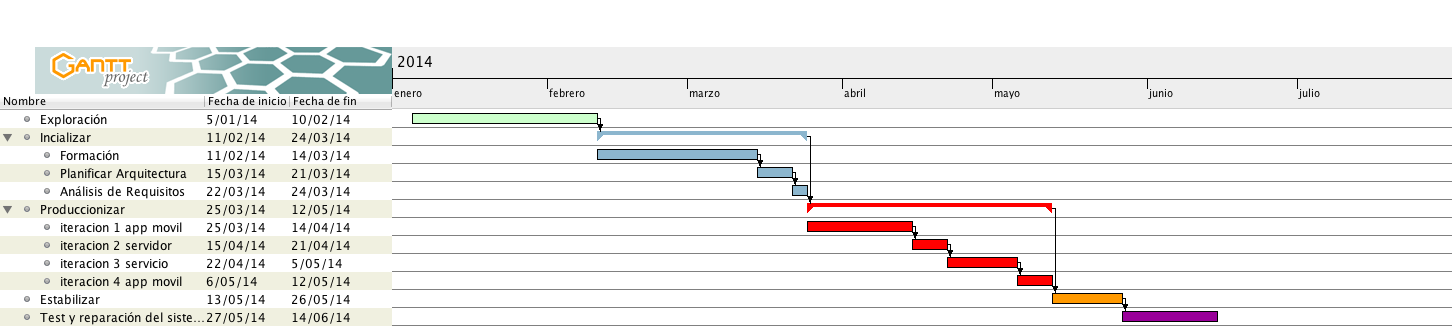
\includegraphics[angle=90,scale=0.45]{diagramagantt.png}
  \caption{Diagrama de Gantt (versión 1.0)}
\end{figure}